\documentclass{beamer}

\usepackage[slovene]{babel}
\usepackage[utf8]{inputenc}
\usepackage{graphicx} % za slike, grafiko
\usepackage{lmodern}
\usepackage{array} % določili <{...} in >{...} pri tabelah
\usepackage{tikz} % za risanje

\usetheme{CambridgeUS}
\usecolortheme{default}
% \useinnertheme[shadows]{rounded}  
\useoutertheme{infolines} % glava in noga

% pisava
\usepackage{palatino}
\usefonttheme{serif}

% definicije in izreki
\newtheorem{definicija}{Definicija}
\newtheorem{izrek}{Izrek}

\begin{document}
% ===================================================================

\title{Priprava prosojnic v \LaTeX-u}
\subtitle{Uporaba paketa beamer}
\author{Ime Priimek}
\institute{FMF}
\date{}

\begin{frame}
\titlepage
\end{frame}
% -------------------------------------------------------------------
\begin{frame}
	\begin{enumerate}
	\frametitle{Kratek pregled}
	\item
	Razporeditev vsebine
\end{enumerate}
\end{frame}

% ===================================================================
\begin{frame}
	\begin{enumerate}
	\frametitle{Kratek pregled}
	\item
	Razporeditev vsebine
	\item
	Matematične trditve
\end{enumerate}
\end{frame}

\begin{frame}
	\begin{enumerate}
	\frametitle{Kratek pregled}
	\item
	Razporeditev vsebine
	\item
	Matematične trditve
	\item
	Postopno odkrivanje vsebine
\end{enumerate}
\end{frame}

\begin{frame}
	\begin{enumerate}
	\frametitle{Kratek pregled}
	\item
	Razporeditev vsebine
	\item
	Matematične trditve
	\item
	Postopno odkrivanje vsebine
	\item
	Razno
\end{enumerate}
\end{frame}

% -------------------------------------------------------------------
\section{Razporeditev vsebine}
\begin{frame}
\frametitle{Naštevanje}
Za naštevanje lahko uporabimo okolje \texttt{itemize:}
\begin{itemize}
\item
      Prva točka.
      \item
      Druga točka.
      \item
      Tretja točka.
\end{itemize}
   ali pa okolje \texttt{enumerate:}
\begin{enumerate}
\item
      Prva točka.
      \item
      Druga točka.
      \item
      Tretja točka.
      \end{enumerate}
\end{frame}

% -------------------------------------------------------------------
\begin{frame}
   \frametitle{Bloki z naslovom}
   Dele besedila lahko zapišemo v bloke.
   Uporabimo okolja \texttt{block, exampleblock, alertblock.}
   Za parameter okolja napišemo naslov bloka.
\begin{block}{Opomba}
      Tako je videti \texttt{block} z naslovom.
\end{block}
\begin{exampleblock}{Primer}
      Tako je videti \texttt{exampleblock} z naslovom.
\end{exampleblock}
\begin{alertblock}{Opozorilo}
      Tako je videti \texttt{alertblock} z naslovom.
\end{alertblock}
\end{frame}

% -------------------------------------------------------------------
\begin{frame}
\frametitle{Bloki brez naslova}
   Blok lahko ima tudi prazen naslov.
   V takem primeru bo brez naslovne vrstice.
   \begin{block}{}
      Tako je videti \texttt{block} s praznim naslovom.
      \end{block}
      \begin{exampleblock}{}
      Tako je videti \texttt{exampleblock} s praznim naslovom.
      \end{exampleblock}
      \begin{alertblock}{}
      Tako je videti \texttt{alertblock} s praznim naslovom.
      \end{alertblock}
\end{frame}

% -------------------------------------------------------------------
\begin{frame}
	\frametitle{Stolpci}
	\begin{columns}
		\begin{column}{0.5 \textwidth}
		\begin{itemize}
\item
            Besedilo lahko pišemo v več stolpcih.
            \item
            Osnovno okolje je \texttt{columns.}
            \item
            Posamezen stolpec opišemo v okolju \texttt{column.}
            \item
            Vsebina stolpca je lahko poljubna.
            \item
            Za primer imamo v desnem stolpcu napis v bloku in sliko sončnice.
            	\end{itemize}
		\end{column}
		
		\begin{column}{0.5 \textwidth}
		\begin{exampleblock}{}
		\centering
Slika v stolpcu
		\end{exampleblock}
		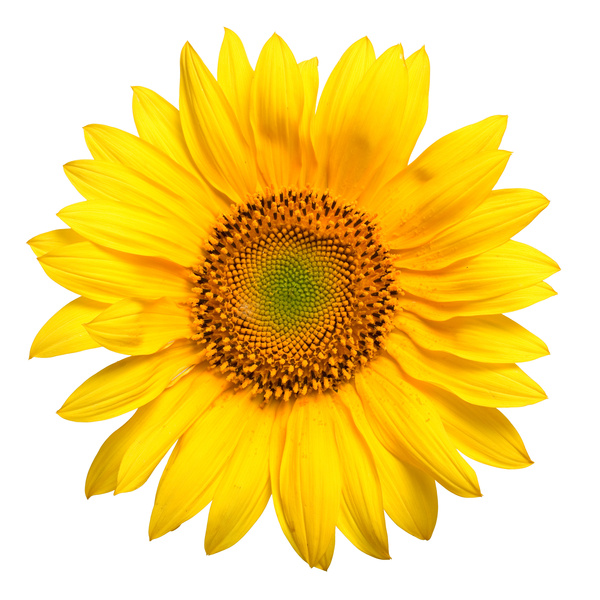
\includegraphics{soncnica.jpg}
		\end{column}
\end{columns}

\end{frame}

% ===================================================================

\section{Matematične trditve}

% -------------------------------------------------------------------
\begin{frame}
\frametitle{Praštevila}

\begin{definicija}
   
      Praštevilo je naravno število, ki ima natanko dva delitelja.
      \end{definicija}
\begin{exampleblock}{Zgledi}     
   	\begin{itemize}
   	\item
         1 je praštevilo (ima samo enega delitelja: 1).
         \item
         2 je praštevilo (ima dva delitelja: 1 in 2).
         \item
         3 je praštevilo (ima dva delitelja: 1 in 3).
         \item
         4 ni praštevilo (ima tri delitelje: 1, 2 in 4).
         \end{itemize}
\end{exampleblock}
\end{frame}
% -------------------------------------------------------------------
\begin{frame}
   \frametitle{Praštevila}
   \begin{izrek}
      Praštevil je neskončno mnogo.
      \end{izrek}
      
      \begin{proof}
      Denimo, da je praštevil končno mnogo.
      \begin{itemize}
      \item
         Naj bo $p$ največje praštevilo.
         \item
         Naj bo $q$ produkt števil 1, 2,$\ldots$, $p$.
         \item
         Število $q+1$ ni deljivo z nobenim praštevilom, torej je $q+1$ praštevilo.
         \item
         To je protislovje, saj je $q+1>p$.
         \end{itemize}
         \end{proof}
\end{frame}

% ===================================================================

\section{Postopno odkrivanje vsebine}

% -------------------------------------------------------------------
\begin{frame}
\frametitle {Konstrukcija pravokotnice na premico p skozi točko T}
\begin{columns}
\begin{column}{0.5 \textwidth}
\begin{itemize}
\item<1->
            Dani sta premica p in točka T.
            \item<2->
            Nariši lok k s središčem v T.
            \item<3->
            Premico p seče v točkah A in B.
            \item<4->
            Nariši lok m s središčem v A.
            \item<5->
            Nariši lok n s središčem v B in z enakim polmerom.
            \item<6->
            Loka se sečeta v točki C.
            \item<7->
            Premica skozi točki T in C je pravokotna na p.
\end{itemize}
\end{column}

\begin{column}{0.5 \textwidth}
\includegraphics<1>[height = 4cm]{pic1.png}
\includegraphics<2>[height = 4cm]{pic2.png}
\includegraphics<3>[height = 4cm]{pic3.png}
\includegraphics<4>[height = 4cm]{pic4.png}
\includegraphics<5>[height = 4cm]{pic5.png}
\includegraphics<6>[height = 4cm]{pic6.png}
\includegraphics<7>[height = 4cm]{pic7.png}

\end{column}

\end{columns}
\end{frame}
% -------------------------------------------------------------------
\begin{frame}
\frametitle{Odkrivanje tabele po vrsticah}
\begin{table}
\begin{tabular}{c| c c c c}

\onslide<1->

      Oznaka& A& B& C& D \onslide<2->  \\  \hline

      X& 1& 2& 3& 4\onslide<3->  \\
      Y& 3& 4& 5& 6 \onslide<4-> \\
      Z& 5& 6& 7& 8 

\end{tabular}
\end{table}
\end{frame}
% -------------------------------------------------------------------
\begin{frame}
\frametitle{Odkrivanje tabele po stolpcih}   
\begin{table}
\begin{tabular}{c |!{\onslide<2->} c!{\onslide<3->} c!{ \onslide<4->}c!{\onslide<5->} c!{\onslide}}

      Oznaka& A& B& C& D \\ \hline
      X& 1& 2& 3& 4 \\
      Y& 3& 4& 5& 6 \\
      Z& 5& 6& 7& 8 \\

\end{tabular}
\end{table}
\end{frame}
% ===================================================================

Razno

% -------------------------------------------------------------------

% ===================================================================

\end{document}